\section{Fase I: Comunicación}

La fase de comunicación, denominada también fase de Inicio o Concepción en el Proceso Unificado Ágil (AUP), representa el punto de partida fundamental de todo el ciclo de vida del software. Según lo establece Roger S. Pressman en su obra \textit{Ingeniería del Software: Un enfoque práctico}, esta actividad estructural tiene como objetivo principal fomentar la colaboración entre el equipo de desarrollo y los interesados (\textit{stakeholders}) para comprender las necesidades reales de la tienda comercializadora y de los clientes que utilizarán la plataforma.

Para el proyecto ``Sistema Web de Compra de Materiales de Escritorio para la empresa Suministros G\&T'', esta fase se orienta bajo el modelo de negocio B2C (\textit{Business to Consumer}), permitiendo que la empresa ofrezca sus productos directamente a clientes particulares a través de una tienda virtual. Mediante un proceso riguroso de indagación y análisis, se identifican los actores involucrados, se establecen los requerimientos funcionales y no funcionales, se definen los términos clave del dominio y se modela el comportamiento general del sistema mediante casos de uso.

\subsection{Identificación de Actores}

Un actor representa cualquier entidad externa (persona, departamento o sistema) que interactúa directamente con la plataforma o que posee un interés directo en su funcionamiento y resultados. Para el sistema web de ``Suministros G\&T'', se han identificado y clasificado los siguientes actores principales y de contexto:

\begin{itemize}
    \item \textbf{Cliente (Comprador Particular u Oficinista):} Es el actor principal del modelo B2C. Representa a la persona natural que accede a la tienda virtual para registrarse, iniciar sesión, consultar el catálogo digital, buscar materiales de escritorio (cuadernos, bolígrafos, papel, archivadores, etc.), revisar características y precios actualizados, administrar su carrito de compras y confirmar pedidos de manera segura.
    \item \textbf{Administrador del Sistema (Gerente de Tienda o Encargado de Inventario):} Es el responsable de gestionar la operatividad comercial de la plataforma. Cuenta con privilegios elevados para registrar, modificar o desactivar productos, organizar categorías, actualizar precios y existencias (\textit{stock}) en tiempo real, administrar cuentas de usuario y supervisar el flujo y estado de los pedidos realizados por los clientes.
    \item \textbf{Proveedor (Actor Externo de Contexto):} Aunque no interactúa directamente con la interfaz del software, constituye una entidad fundamental en el ecosistema del negocio al abastecer de materiales a ``Suministros G\&T''. El sistema refleja este flujo mediante el control de inventario para garantizar la disponibilidad física de los artículos ofertados.
    \item \textbf{Equipo de Desarrollo (Analistas, Diseñadores y Programadores):} Los integrantes del equipo de Ingeniería de Software actúan como los responsables de analizar, diseñar, construir y documentar la solución técnica, asegurando el cumplimiento de los estándares de calidad y los plazos establecidos.
    \item \textbf{Docente de la Asignatura (Cliente Académico / Evaluador):} Actúa como \textit{stakeholder} auditor del proceso, verificando que la aplicación de las metodologías de ingeniería de software (AUP y Pressman) se ejecute de forma rigurosa y debidamente documentada.
\end{itemize}

\subsection{Requerimientos Funcionales y No Funcionales}

A través del análisis del negocio se han extraído y codificado los requerimientos del sistema para garantizar su trazabilidad durante todo el ciclo de desarrollo.

\subsubsection{Requerimientos Funcionales (RF)}

Los requerimientos funcionales describen las operaciones, validaciones y servicios específicos que la plataforma debe ofrecer a sus usuarios:

\begin{itemize}
    \item \textbf{RF01 (Registro de clientes):} El sistema permitirá a los nuevos usuarios crear una cuenta mediante un formulario, registrando y validando sus datos básicos (nombre, correo electrónico, dirección, teléfono y contraseña).
    \item \textbf{RF02 (Inicio y cierre de sesión):} El sistema permitirá a los usuarios registrados (clientes y administradores) autenticarse mediante credenciales válidas, redirigiéndolos a su entorno correspondiente, así como cerrar su sesión de forma segura.
    \item \textbf{RF03 (Gestión de perfiles):} El cliente autenticado podrá consultar su información personal y actualizar datos como su dirección, teléfono o contraseña.
    \item \textbf{RF04 (Catálogo digital de productos):} El sistema mostrará un catálogo digital organizado con los materiales de escritorio disponibles en la tienda (cuadernos, bolígrafos, lápices, hojas bond, carpetas, archivadores, marcadores, entre otros).
    \item \textbf{RF05 (Clasificación por categorías):} El sistema permitirá filtrar y navegar los productos agrupados en categorías lógicas para facilitar su localización.
    \item \textbf{RF06 (Búsqueda de productos):} El cliente podrá buscar artículos específicos ingresando palabras clave, nombre del producto o categoría en un buscador interno.
    \item \textbf{RF07 (Detalle del producto):} Al seleccionar un artículo, el cliente podrá visualizar una ficha informativa con su nombre, descripción detallada, características, precio unitario, imagen referencial y disponibilidad (\textit{stock}).
    \item \textbf{RF08 (Carrito de compras):} El sistema permitirá al cliente seleccionar la cantidad deseada de un producto y agregarlo a un carrito de compras virtual.
    \item \textbf{RF09 (Modificación del carrito):} El cliente podrá modificar las cantidades de los artículos añadidos al carrito o eliminarlos antes de confirmar su pedido.
    \item \textbf{RF10 (Cálculo automático de importes):} El sistema calculará en tiempo real los subtotales por cada producto y el monto total general de la compra conforme se modifica el carrito.
    \item \textbf{RF11 (Validación de disponibilidad):} El sistema validará que las cantidades solicitadas sean válidas y que exista \textit{stock} suficiente en el inventario antes de permitir la confirmación de un pedido.
    \item \textbf{RF12 (Confirmación y registro de pedidos):} El cliente podrá revisar el resumen de su compra y confirmar el pedido, generando un registro único con el detalle de productos, cantidades, precios, fecha y datos del comprador, descontando automáticamente las existencias.
    \item \textbf{RF13 (Historial y seguimiento de pedidos):} El cliente podrá consultar su historial de compras realizadas y visualizar el estado actual de sus pedidos vigentes (ej. ``Recibido'', ``En preparación'', ``En camino'', ``Entregado'').
    \item \textbf{RF14 (Administración de productos):} El administrador contará con un módulo para registrar nuevos productos, consultar y modificar los existentes (precios, descripciones, imágenes) y desactivar aquellos que ya no se comercialicen.
    \item \textbf{RF15 (Administración de categorías):} El administrador podrá crear, modificar, organizar y desactivar las categorías de productos del catálogo.
    \item \textbf{RF16 (Gestión de precios e inventario):} El administrador podrá actualizar los precios y reabastecer las existencias (\textit{stock}) de los materiales para mantener la sincronía con el almacén físico.
    \item \textbf{RF17 (Gestión de pedidos):} El administrador podrá consultar todos los pedidos realizados por los clientes, revisar su detalle y actualizar su estado de atención y entrega.
    \item \textbf{RF18 (Gestión de usuarios):} El administrador podrá consultar el listado de clientes registrados y administrar el estado de sus cuentas dentro de la plataforma.
\end{itemize}

\subsubsection{Requerimientos No Funcionales (RNF)}

Los requerimientos no funcionales establecen los atributos de calidad, restricciones técnicas y estándares de operación que debe cumplir la plataforma:

\begin{itemize}
    \item \textbf{RNF01 (Usabilidad):} La interfaz debe ser clara, ordenada e intuitiva, aplicando principios de diseño UX/UI para facilitar la navegación y minimizar la curva de aprendizaje tanto para clientes como para administradores.
    \item \textbf{RNF02 (Rendimiento):} Las consultas al catálogo, búsquedas y operaciones del carrito deberán responder en tiempos óptimos (menores a 3 segundos en condiciones normales) para brindar una experiencia fluida.
    \item \textbf{RNF03 (Seguridad y control de acceso):} El sistema protegerá el acceso mediante autenticación robusta y restringirá las funciones administrativas exclusivamente a usuarios con el rol autorizado.
    \item \textbf{RNF04 (Privacidad y protección de datos):} Las contraseñas y datos personales de los clientes se almacenarán de forma cifrada y se utilizarán únicamente para las operaciones propias de la tienda virtual.
    \item \textbf{RNF05 (Disponibilidad):} La plataforma deberá mantenerse operativa y accesible durante el horario de atención de la tienda, minimizando interrupciones en el servicio.
    \item \textbf{RNF06 (Compatibilidad):} La aplicación web deberá funcionar correctamente en los principales navegadores modernos (Google Chrome, Mozilla Firefox, Microsoft Edge, Safari).
    \item \textbf{RNF07 (Adaptabilidad / \textit{Responsive Design}):} La interfaz se adaptará automáticamente a distintos tamaños de pantalla, permitiendo su uso en computadoras de escritorio, tabletas y teléfonos móviles.
    \item \textbf{RNF08 (Integridad de datos):} La información de productos, precios, existencias y pedidos deberá mantenerse consistente mediante validaciones estrictas antes de persistir cambios en la base de datos.
    \item \textbf{RNF09 (Mantenibilidad):} El sistema se estructurará de forma modular y documentada para facilitar futuras correcciones, mantenimiento y ampliaciones de funcionalidad.
    \item \textbf{RNF10 (Respaldo de información):} Se implementarán copias de seguridad (\textit{backups}) periódicas de la base de datos para prevenir la pérdida de información crítica ante fallos.
    \item \textbf{RNF11 (Escalabilidad):} La arquitectura permitirá incorporar futuras mejoras (como pasarelas de pago electrónico o reportes avanzados) sin comprometer el rendimiento general.
\end{itemize}

\subsection{Glosario de Términos Técnicos}

Con el propósito de unificar el lenguaje entre los interesados del negocio y el equipo técnico, en la Tabla \ref{tab:glosario_terminos} se definen los conceptos fundamentales del proyecto.

{\small
\begin{xltabular}{\textwidth}{|>{\raggedright\arraybackslash}p{4.2cm}|X|}
    % --- Título y encabezado de la PRIMERA página ---
    \caption{Glosario de términos técnicos y del dominio del negocio}
    \label{tab:glosario_terminos} \\
    \hline
    \textbf{Término} & \textbf{Definición} \\
    \hline
    \endfirsthead

    % --- Encabezado que se repite en las páginas SIGUIENTES ---
    \multicolumn{2}{l}{\textit{Continuación de la Tabla \ref{tab:glosario_terminos}}} \\
    \hline
    \textbf{Término} & \textbf{Definición} \\
    \hline
    \endhead

    % --- Pie de tabla en páginas intermedias ---
    \multicolumn{2}{r}{\textit{Continúa en la siguiente página...}} \\
    \endfoot

    % --- Pie final de la tabla ---
    \endlastfoot

    % --- Contenido de las filas ---
    AUP (\textit{Agile Unified Process}) & Proceso de desarrollo de software ágil y simplificado que aplica técnicas de modelado y gestión iterativa. \\
    \hline
    B2C (\textit{Business to Consumer}) & Modelo de negocio en el que una empresa comercializa productos o servicios directamente al consumidor final por internet. \\
    \hline
    Cliente-Servidor & Arquitectura de software donde el cliente (navegador web) solicita recursos o servicios al servidor que aloja la lógica y los datos. \\
    \hline
    Frontend / Backend & El \textit{Frontend} es la interfaz visual con la que interactúa el usuario; el \textit{Backend} gestiona la lógica de negocio, seguridad y base de datos. \\
    \hline
    Tienda virtual / Sistema web & Plataforma digital accesible mediante un navegador web que permite exhibir productos y gestionar compras en línea. \\
    \hline
    Catálogo digital & Listado estructurado de los materiales de escritorio disponibles para su consulta en la plataforma. \\
    \hline
    Categoría & Clasificación lógica que agrupa productos con características o usos similares dentro del catálogo. \\
    \hline
    Producto & Artículo de escritorio ofertado para la venta, con atributos como nombre, descripción, precio, imagen y disponibilidad. \\
    \hline
    Carrito de compras & Espacio virtual temporal donde el cliente reúne y ajusta los productos que desea adquirir antes de confirmar su pedido. \\
    \hline
    Pedido & Registro formal de una compra confirmada por el cliente, que detalla los artículos, cantidades solicitadas, importes y estado. \\
    \hline
    Existencias (\textit{Stock}) & Cantidad física disponible de un producto en almacén para su comercialización. \\
    \hline
    Autenticación y Roles & Proceso de verificación de identidad del usuario y asignación de permisos según su perfil (Cliente o Administrador). \\
    \hline
    Base de datos & Repositorio estructurado que almacena de forma íntegra la información de usuarios, productos, categorías, inventarios y pedidos. \\
    \hline
    UML y Casos de Uso & Lenguaje Unificado de Modelado utilizado para representar gráficamente las interacciones entre los actores y las funciones del sistema. \\
    \hline
    UX/UI y \textit{Responsive} & Disciplinas enfocadas en la experiencia e interfaz de usuario, garantizando una navegación intuitiva y adaptable a cualquier pantalla. \\
    \hline
\end{xltabular}
}

\subsection{Modelado de Casos de Uso Generales del Sistema}

El modelado de casos de uso representa las principales funcionalidades que ofrece la tienda virtual desde la perspectiva de los actores que interactúan con ella. Cabe señalar que, dentro del alcance definido para esta versión, no se incluye una pasarela de pagos electrónicos como actor externo obligatorio, ya que el flujo se centra en la gestión del catálogo, carrito y confirmación de pedidos.

% =========================================================================
% INICIO DE BLOQUE PARA IMAGEN: DIAGRAMA DE CASOS DE USO GENERAL
% Descomenta las siguientes líneas y reemplaza "diagrama_casos_uso.png"
% con el nombre real de tu archivo de imagen (en formato PNG, JPG o PDF).
% =========================================================================
% \begin{figure}[htbp]
%     \centering
%     \includegraphics[width=0.95\textwidth]{diagrama_casos_uso.png}
%     \caption{Diagrama de Casos de Uso General del Sistema Web de Compra de Materiales de Escritorio (B2C)}
%     \label{fig:casos_uso_general}
% \end{figure}
% =========================================================================
% FIN DE BLOQUE PARA IMAGEN
% =========================================================================
\begin{figure}[htbp]
    \centering
    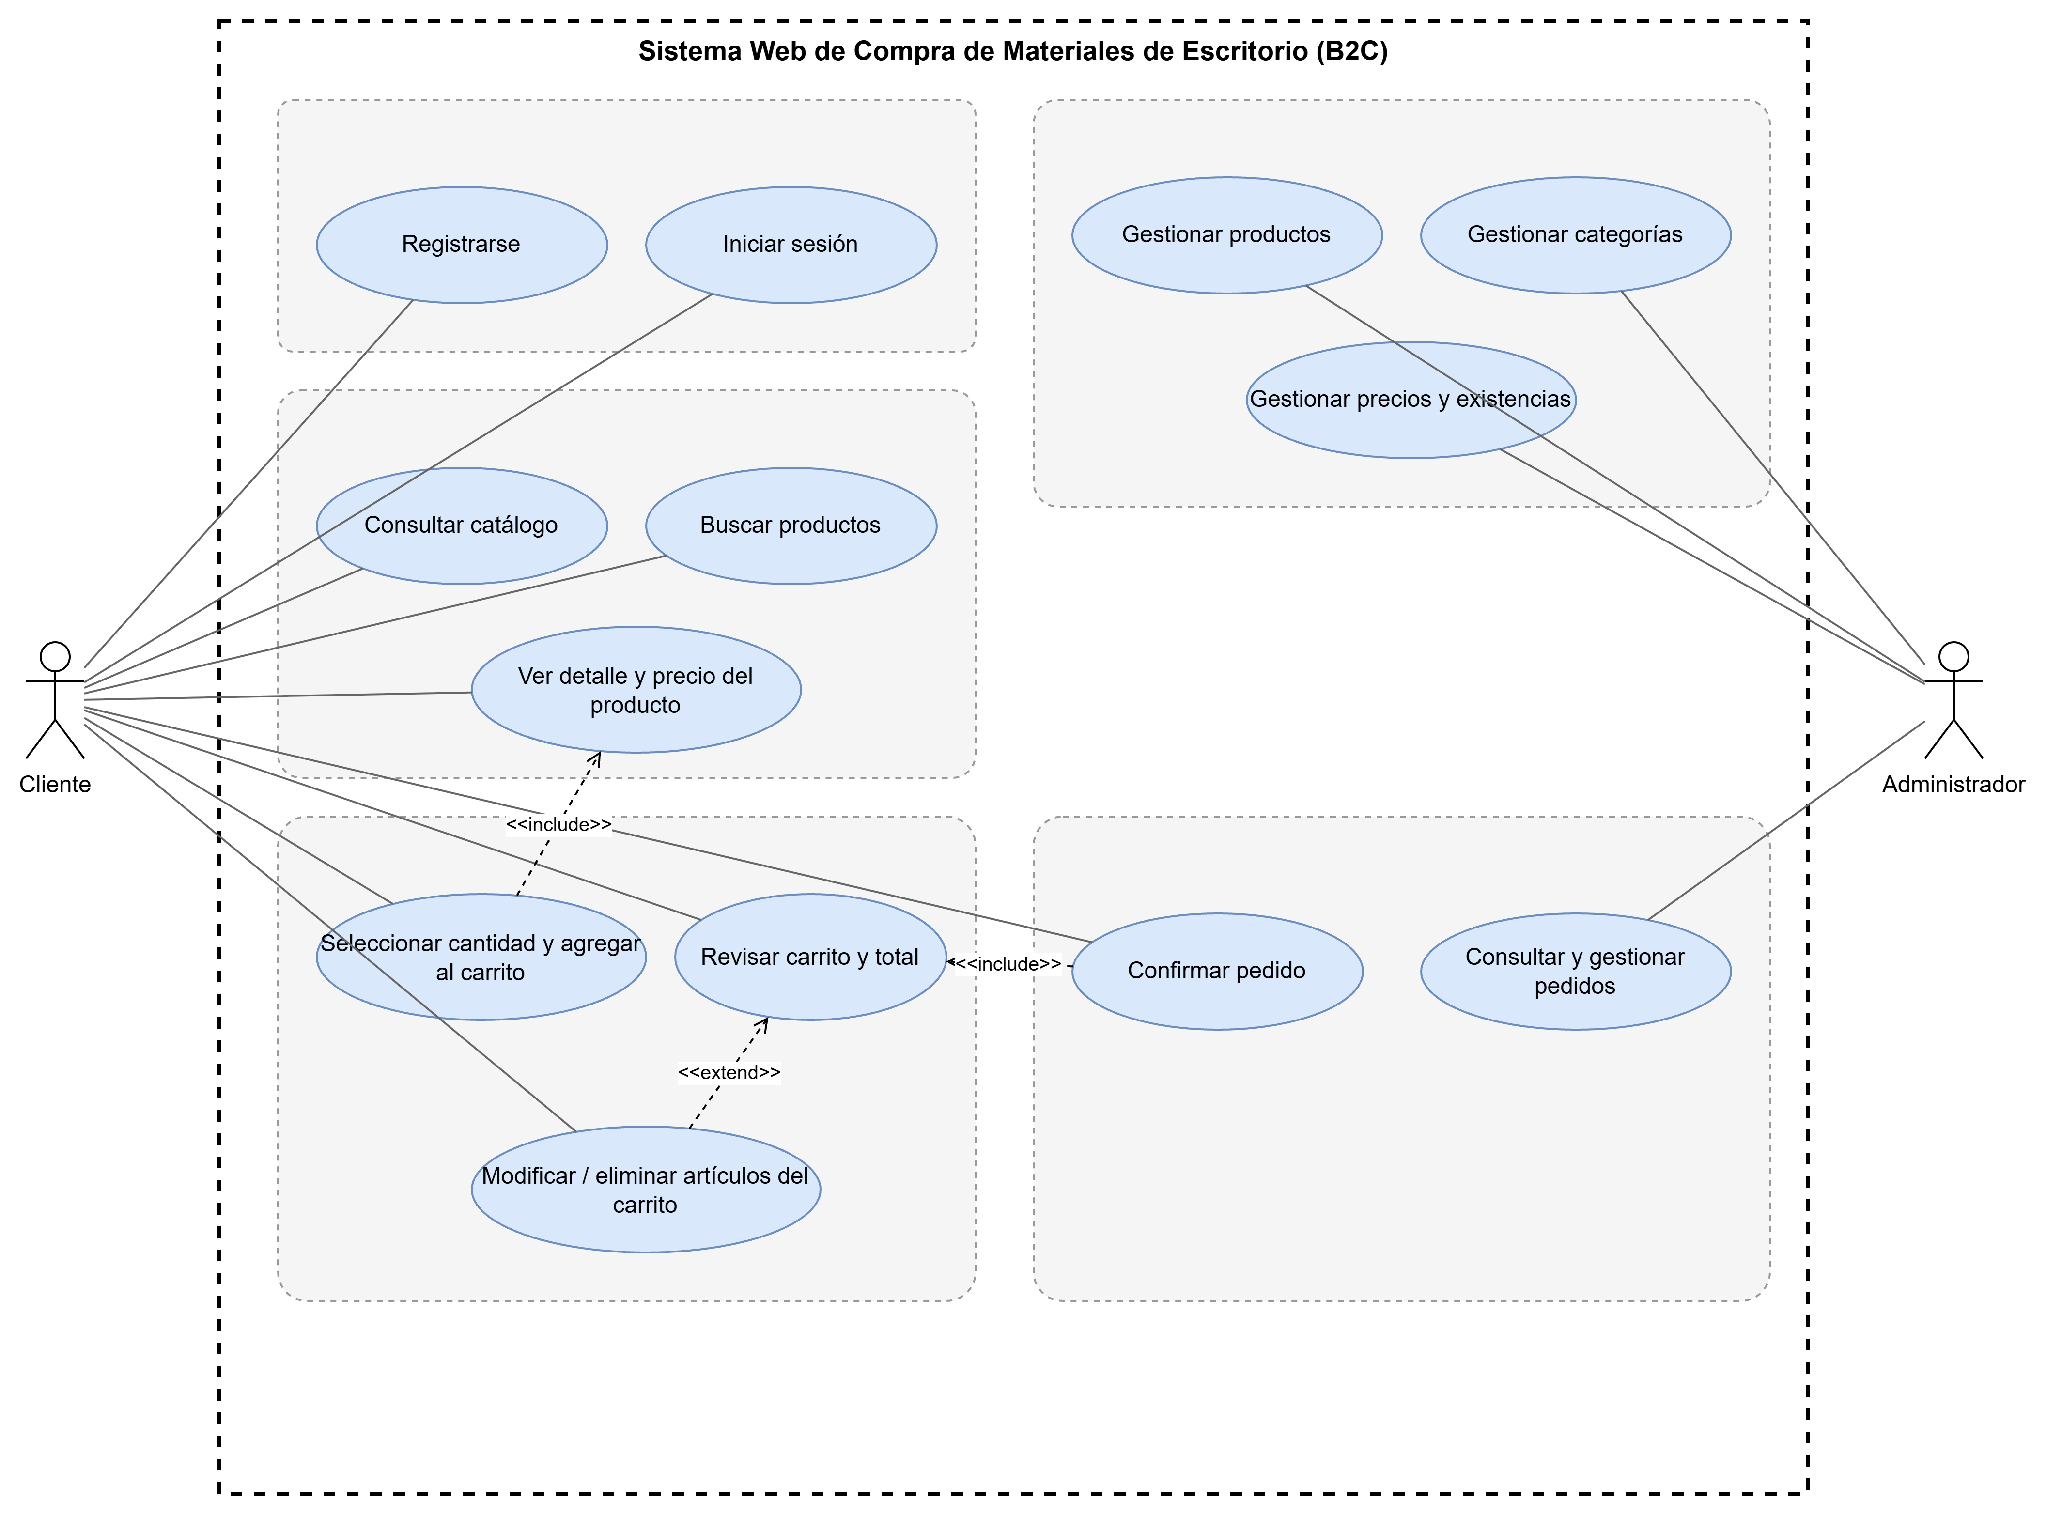
\includegraphics[width=1\textwidth]{diagrama_general.png}
    \caption{Diagrama de Casos de Uso General del Sistema Web de Compra de Materiales de Escritorio (B2C)}
    \label{fig:casos_uso_general}
\end{figure}
Como se ilustra en el diagrama general del sistema, el \textbf{Cliente} interactúa con los casos de uso de registro, inicio de sesión, consulta y búsqueda en el catálogo, visualización de detalles, gestión del carrito de compras (con relaciones \texttt{<<include>>} hacia la consulta de detalle y \texttt{<<extend>>} para modificar o eliminar artículos) y confirmación de pedidos. Por su parte, el \textbf{Administrador} gestiona productos, categorías, precios, existencias y la atención de pedidos.

A continuación, se detallan las especificaciones de los escenarios principales del sistema:

\subsubsection*{Caso de Uso 01: Gestionar Carrito de Compras y Confirmar Pedido}
\begin{itemize}
    \item \textbf{Actor Principal:} Cliente.
    \item \textbf{Precondición:} El cliente debe haber iniciado sesión (RF02) y estar visualizando el catálogo digital (RF04).
    \item \textbf{Flujo Normal:}
    \begin{enumerate}
        \item El cliente selecciona un producto del catálogo y pulsa la opción ``Agregar al carrito'' (RF08).
        \item El sistema verifica la disponibilidad de \textit{stock} en el inventario (RF11).
        \item El sistema añade el artículo al carrito y actualiza el contador de productos.
        \item El cliente ingresa al resumen del carrito, revisa los artículos seleccionados y modifica la cantidad de alguno de ellos (RF09).
        \item El sistema recalcula automáticamente los subtotales y el monto total a pagar (RF10).
        \item El cliente presiona ``Confirmar Pedido'' (RF12).
        \item El sistema valida nuevamente las existencias, genera un identificador único de pedido, descuenta el \textit{stock} del inventario y muestra un mensaje de confirmación.
    \end{enumerate}
    \item \textbf{Flujo Alternativo (Falta de Stock):} En el paso 2 o 7, si el sistema detecta que la cantidad solicitada supera las existencias disponibles, bloquea la operación y notifica al cliente que el producto se encuentra agotado o con unidades limitadas.
\end{itemize}

\subsubsection*{Caso de Uso 02: Gestionar Catálogo e Inventario}
\begin{itemize}
    \item \textbf{Actor Principal:} Administrador del Sistema.
    \item \textbf{Precondición:} El administrador ha iniciado sesión con sus credenciales autorizadas (RNF03).
    \item \textbf{Flujo Normal:}
    \begin{enumerate}
        \item El administrador accede al panel de administración de productos.
        \item Selecciona la opción ``Registrar nuevo producto'' (RF14).
        \item El sistema despliega el formulario de registro.
        \item El administrador completa los campos requeridos (nombre, categoría, descripción, precio unitario, \textit{stock} inicial e imagen referencial).
        \item El administrador pulsa ``Guardar''.
        \item El sistema valida la integridad de los datos (RNF08), almacena el registro en la base de datos y actualiza el catálogo visible para los clientes.
    \end{enumerate}
    \item \textbf{Flujo Alternativo (Datos Inválidos o Incompletos):} En el paso 6, si algún campo obligatorio (como el precio o el nombre) está vacío o contiene un formato incorrecto, el sistema resalta el campo y solicita su corrección antes de guardar.
\end{itemize}

\subsubsection*{Caso de Uso 03: Consultar y Actualizar Estado de Pedido}
\begin{itemize}
    \item \textbf{Actor Principal:} Cliente / Administrador del Sistema.
    \item \textbf{Precondición:} Existe al menos un pedido registrado previamente en el sistema (RF12).
    \item \textbf{Flujo Normal:}
    \begin{enumerate}
        \item El cliente ingresa a la sección ``Mis Pedidos'' en su perfil para consultar su historial (RF13), mientras que el administrador accede al módulo de ``Gestión de Pedidos'' (RF17).
        \item El administrador selecciona un pedido entrante, verifica los artículos solicitados y actualiza su estado (por ejemplo, de ``Recibido'' a ``En preparación'' o ``Entregado'').
        \item El sistema registra el cambio de estado y lo refleja en tiempo real en la vista de seguimiento del cliente.
    \end{enumerate}
\end{itemize}

\subsection{Evaluación de la Fase de Comunicación}

Al concluir las actividades de la Fase I bajo el enfoque metodológico AUP, el equipo de desarrollo establece las siguientes conclusiones evaluativas:

\begin{itemize}
    \item \textbf{Viabilidad técnica y operativa:} El proyecto es plenamente viable. La solución web bajo el modelo B2C responde directamente a la necesidad de digitalizar el catálogo de ``Suministros G\&T'', agilizar la toma de pedidos y reducir la dependencia de procesos manuales.
    \item \textbf{Calidad y trazabilidad de requerimientos:} Se definieron 18 requerimientos funcionales y 11 no funcionales claros, medibles y codificados, evitando ambigüedades mediante métricas concretas (como tiempos de respuesta y validaciones de inventario).
    \item \textbf{Delimitación temprana del alcance:} Se acordó desde esta etapa inicial que la primera versión del sistema no integrará pasarelas de pago en línea ni rastreo satelital de entregas, evitando desviaciones de alcance (\textit{scope creep}) y alineando las expectativas entre el equipo y el negocio.
    \item \textbf{Consenso y base documental:} La elaboración del glosario técnico y la especificación de los casos de uso proporcionan una base sólida y libre de ambigüedades para avanzar hacia las siguientes fases de Planeación y Modelado.
\end{itemize}
